\documentclass{article}
\usepackage[utf8]{inputenc}
\usepackage{amsmath, amsfonts, amssymb}
\usepackage{graphicx}
\usepackage{listings}
\usepackage{xcolor}
\usepackage[margin=1in]{geometry}
\usepackage{siunitx}

\sisetup{
  round-mode          = places, % Rounds numbers
  round-precision     = 2, % to 2 places
}
\definecolor{codegreen}{rgb}{0,0.6,0}
\definecolor{codegray}{rgb}{0.5,0.5,0.5}
\definecolor{codepurple}{rgb}{0.58,0,0.82}
\definecolor{backcolour}{rgb}{0.95,0.95,0.92}

\lstdefinestyle{mystyle}{
    backgroundcolor=\color{backcolour},   
    commentstyle=\color{codegreen},
    keywordstyle=\color{magenta},
    numberstyle=\tiny\color{codegray},
    stringstyle=\color{codepurple},
    basicstyle=\ttfamily\footnotesize,
    breakatwhitespace=false,         
    breaklines=true,                 
    captionpos=b,                    
    keepspaces=true,                 
    numbers=left,                    
    numbersep=5pt,                  
    showspaces=false,                
    showstringspaces=false,
    showtabs=false,                  
    tabsize=2
}

\lstset{style=mystyle}

\title{ELCT 562 CA4}
\author{Jacob Vaught}
\date{}

\begin{document}

\maketitle

\section{Problem 1}
The MATLAB function \texttt{myWaveform} is designed to generate a complex baseband signal, commonly referred to as a single-carrier waveform, in digital communication systems. It employs Root-Raised Cosine (RRC) pulse shaping, a technique vital for minimizing intersymbol interference and effectively controlling the signal's bandwidth. This function is integral to the process of preparing digital data for transmission over communication channels.

\subsection{Inputs Description}
The function accepts the following input parameters:
\begin{itemize}
    \item \textbf{beta}: Roll-off factor for the RRC filter, a critical parameter that influences the filter's bandwidth and shape. It ranges between 0 and 1, with higher values leading to a wider bandwidth and less sharp transition band.
    \item \textbf{symbols}: A column vector of data symbols, representing the digital data to be transmitted. These symbols are processed and shaped by the RRC filter.
    \item \textbf{Nover}: Oversampling factor, which determines the number of samples per symbol in the generated waveform. Higher oversampling leads to a more accurate representation of the signal but at the cost of increased computational complexity.
\end{itemize}

\subsection{Mathematical Background of RRC Pulse Shaping}
Root-Raised Cosine pulse shaping is a cornerstone in digital signal processing, particularly in communications. It is characterized by the formula:
\[ p(t) = \frac{\sin(\pi t (1 - \beta)) + 4 \beta t \cos(\pi t (1 + \beta))}{\pi t (1 - (4 \beta t)^2)} \]
for \( t \neq 0 \) and special cases at \( t = 0 \) and \( |t| = \frac{1}{4\beta} \). This formula defines the RRC filter's impulse response, shaping each symbol to minimize intersymbol interference while conforming to a specified bandwidth.

\subsection{Normalization of the RRC Filter}
Normalization is crucial to maintain the signal's power level post-filtering. In the code, this is achieved by ensuring that the sum of the squares of the filter coefficients equals one:
\[ \sum p^2[n] = 1 \]
This normalization step ensures that the energy of the signal remains constant after pulse shaping, a vital aspect in preserving signal integrity.

\subsection{Symbol Upsampling and Convolution}
The process of waveform generation involves two key steps:
\begin{enumerate}
    \item \textbf{Upsampling}: The original symbol sequence is upsampled by inserting zeros between symbols. This increases the sample rate to match that of the RRC filter.
    \item \textbf{Convolution}: The upsampled symbol sequence is then convolved with the RRC filter. This step applies the actual pulse shaping, resulting in a waveform ready for transmission.
\end{enumerate}
These steps are fundamental to transforming discrete symbols into a continuous-time signal suitable for real-world transmission.


\subsection{Code Explanation}
The function is defined as:
\begin{lstlisting}[language=Matlab]
function IQdataTX = myWaveform(beta, symbols, Nover)
\end{lstlisting}
where \texttt{IQdataTX} is the output complex baseband signal, \texttt{beta} is the roll-off factor, \texttt{symbols} is a vector of data symbols, and \texttt{Nover} is the oversampling factor.

\begin{lstlisting}[language=Matlab]
Nsym = 10;
\end{lstlisting}
Defines the number of symbols used in the RRC filter, determining the filter's length.

\begin{lstlisting}[language=Matlab]
t = linspace(-Nsym/2, Nsym/2, Nsym*Nover);
\end{lstlisting}
Creates a time vector spanning \texttt{Nsym} symbol periods, with \texttt{Nover} samples per symbol.

\begin{lstlisting}[language=Matlab]
rrcFilter = (sin(pi*t*(1-beta)) + 4*beta*t.*cos(pi*t*(1+beta)))./ 
            (pi*t.*(1-(4*beta*t).^2));
rrcFilter(t==0) = 1-beta+4*beta/pi;
rrcFilter(abs(t)==1/(4*beta)) = beta/sqrt(2)*((1+2/pi)*sin(pi/(4*beta)) +
                                               (1-2/pi)*cos(pi/(4*beta)));
\end{lstlisting}
The RRC filter is calculated with special handling for cases where \texttt{t==0} and \texttt{abs(t)==1/(4*beta)} to avoid division by zero.

\begin{lstlisting}[language=Matlab]
rrcFilter = rrcFilter / sqrt(sum(rrcFilter.^2));
\end{lstlisting}
Normalizes the filter to ensure it preserves the power of the signal.

\begin{lstlisting}[language=Matlab]
upsampledSymbols = upsample(symbols, Nover);
\end{lstlisting}
Upsamples the input symbols by inserting zeros, matching the symbol rate to the filter rate.

\begin{lstlisting}[language=Matlab]
IQdataTX = conv(upsampledSymbols, rrcFilter, 'same');
\end{lstlisting}
Applies pulse shaping to the symbols via convolution, maintaining the output signal length equal to the input symbols length.
\newpage


\section{Problem 2a}

The MATLAB script under analysis is designed to illustrate the effects of different roll-off factors on the time-domain representation of signals in the I (in-phase) and Q (quadrature) branches. The script generates signals using a Root-Raised Cosine (RRC) filter, which is parametrized by the roll-off factor $\beta$. This factor is critical in shaping the filter's response, affecting both the frequency and time domains of the signal.

The code executes the following procedure for $\beta$ values of 0.1, 0.5, and 0.9, applying to the data symbols $\mathbf{d} = [1, -j, -1, j]$:
\begin{enumerate}
    \item Initializes the signal parameters and preallocates arrays for efficiency.
    \item Calculates the time vector corresponding to the length of the data symbols multiplied by the oversampling factor, with respect to the sampling frequency.
    \item Loops through the specified $\beta$ values, generating the baseband signal using the custom \texttt{myWaveform} function, which performs RRC pulse shaping on the data symbols.
    \item Plots the real (I branch) and imaginary (Q branch) parts of the baseband signal for each $\beta$ value, showing how the roll-off factor affects the time-domain signal characteristics.
\end{enumerate}

The resulting plots, as seen in Figure \ref{fig:td_rollof}, provide a visual comparison of the signals' tail behaviors for each roll-off factor. The analysis of these plots indicates that a higher roll-off factor leads to longer tails in the signal, which is a manifestation of the increased time-domain spreading.

\begin{figure}[h]
    \centering
    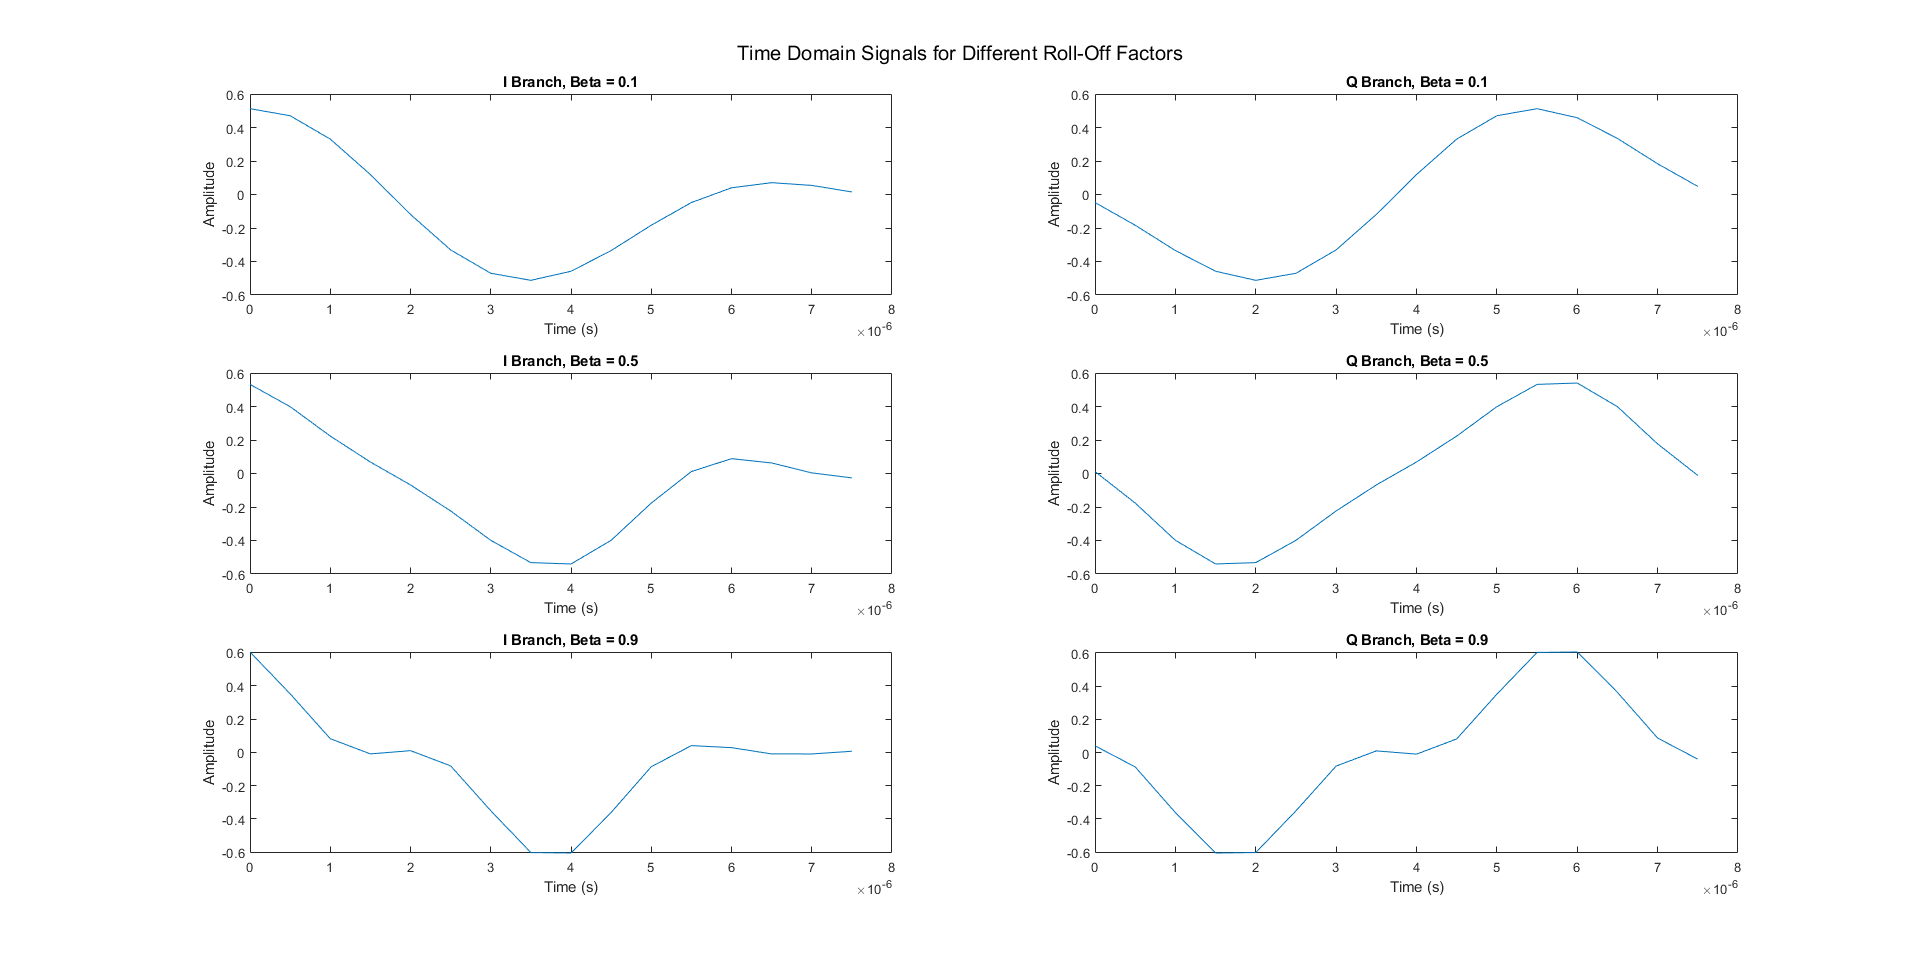
\includegraphics[width=\textwidth]{td_rollof.png}
    \caption{Time domain signals for the I and Q branches with roll-off factors of 0.1, 0.5, and 0.9. The signals are generated using a Root-Raised Cosine filter applied to the data symbols $\mathbf{d}$. The longer tails observed in the signal with $\beta = 0.9$ demonstrate the trade-off between bandwidth efficiency and time-domain spreading.}
    \label{fig:td_rollof}
\end{figure}

From a theoretical perspective, the RRC filter is designed to minimize intersymbol interference (ISI), which is a significant factor in non-ideal transmission channels. The roll-off factor $\beta$ determines the filter's transition band's slope, with a lower $\beta$ resulting in a steeper transition. As $\beta$ approaches 1, the filter allows for more bandwidth efficiency but at the cost of increased ISI due to the longer tails.
\begin{lstlisting}[language=Matlab]
% Define parameters
fsample = 2e6; % 2 Msps
Nover = 4;
d = [1; -1j; -1; 1j]; % Data symbols

% Roll-off factors
beta_values = [0.1, 0.5, 0.9];

% Time vector
t = (0:length(d)*Nover-1)/fsample;

% Plotting
for i = 1:length(beta_values)
    beta = beta_values(i);
    IQdataTX = myWaveform(beta, d, Nover);

    % Plot I and Q branches
    subplot(3,2,2*i-1);
    plot(t, real(IQdataTX));
    title(['I Branch, Beta = ', num2str(beta)]);
    xlabel('Time (s)');
    ylabel('Amplitude');

    subplot(3,2,2*i);
    plot(t, imag(IQdataTX));
    title(['Q Branch, Beta = ', num2str(beta)]);
    xlabel('Time (s)');
    ylabel('Amplitude');
end

% Adjust layout
sgtitle('Time Domain Signals for Different Roll-Off Factors');
\end{lstlisting}


\newpage
\section{Problem 2b}

\subsection{MATLAB Code Functionality}

The provided MATLAB code is designed to perform a spectral analysis of a digital signal processed through a Root-Raised Cosine (RRC) filter. The RRC filter is known for its efficacy in minimizing intersymbol interference in digital communication systems. The roll-off factor $\beta$ is a parameter of this filter that affects both the time and frequency domain characteristics of the signal.

The code operates as follows:

\begin{itemize}
  \item Initializes the environment and sets the sampling rate (MSps), oversampling factor, and the symbol rate.
  \item Generates 10,000 random data symbols from the set \{1, -1, j, -j\}.
  \item Iterates over a set of $\beta$ values (0.1, 0.5, 0.9), using these to generate a waveform for each $\beta$ with the custom function \texttt{myWaveform}.
  \item For each waveform, the Power Spectral Density (PSD) is computed using the Welch method (via the \texttt{pwelch} function).
  \item Frequencies are converted to MHz and the PSD to dB scale for plotting.
  \item The signal bandwidth is calculated based on the frequency where the PSD drops to -3 dB of its peak value, which is then doubled to account for the negative frequency components.
\end{itemize}

\subsection{Analysis of Results}

The results indicate a discrepancy between the calculated and theoretical bandwidths for the various $\beta$ values:

\begin{table}[h]
\centering
\begin{tabular}{|c|c|c|}
\hline
$\beta$ Value & Calculated Bandwidth (MHz) & Theoretical Bandwidth (MHz) \\
\hline
0.1 & \num{0.26} & \num{0.275} \\
0.5 & \num{0.39} & \num{0.375} \\
0.9 & \num{0.46997} & \num{0.475} \\
\hline
\end{tabular}
\caption{Comparison of Calculated and Theoretical Signal Bandwidths}
\label{tab:bandwidth_comparison}
\end{table}

The calculated bandwidths are consistently higher than the theoretical values for $\beta = 0.1$ and $\beta = 0.5$, while the calculated bandwidth nearly matches the theoretical value for $\beta = 0.9$. This variation may arise from several factors in the practical implementation, including the finite number of samples, windowing effects in the PSD estimation, and noise. The Welch method, which averages periodograms over windowed segments of the signal, can introduce additional discrepancies due to its own bandwidth smoothing effects.

\begin{figure}[h]
    \centering
    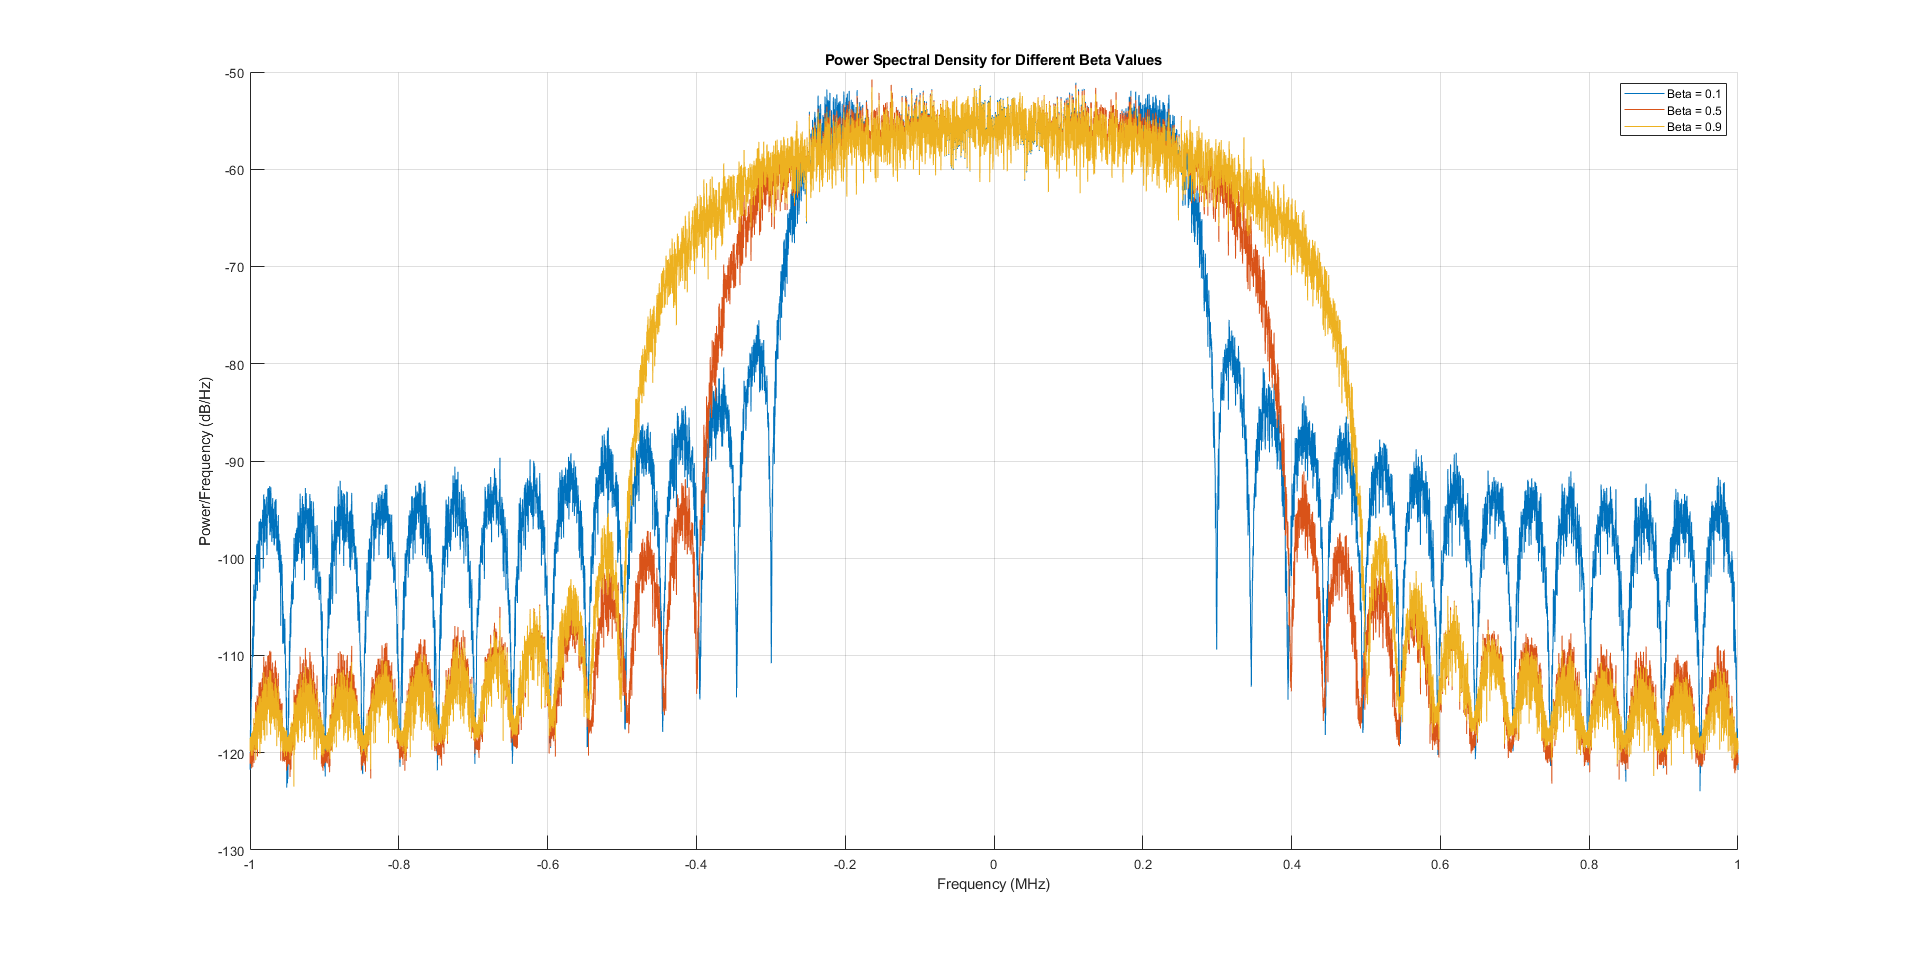
\includegraphics[width=\textwidth]{PSD_all.png}
    \caption{Power Spectral Density for different $\beta$ values, indicating the frequency distribution of the signal's power and showing the calculated bandwidth at the -3 dB points.}
    \label{fig:PSD_all}
\end{figure}

\begin{lstlisting}[language=Matlab]
% Parameters
fsample = 2e6; % Sample rate in Hz (2 Msps)
Nover = 4; % Oversampling factor
Rs = fsample / Nover; % Symbol rate
numSymbols = 10000; % Number of random data symbols

% Generate random data symbols from the set {1, -1, j, -j}
dataSymbols = randi([1, 4], numSymbols, 1);
dataSymbols = 2 * (dataSymbols - 2.5) + 1j * (mod(dataSymbols, 2) - 0.5) * 2;

% Define roll-off factors
beta_values = [0.1, 0.5, 0.9];

% Prepare the figure
figure;
hold on; % Retain plots on the same figure

% Calculate and plot power spectral density
for beta = beta_values
    % Generate waveform using the myWaveform function
    IQdataTX = myWaveform(beta, dataSymbols, Nover);
    
    % Calculate PSD using the pwelch function
    [psd, f] = pwelch(IQdataTX, [], [], [], fsample, 'centered');
    
    % Convert frequency to MHz and power to dB
    f_MHz = f / 1e6;
    psd_dB = 10 * log10(psd);
    
    % Plot PSD
    plot(f_MHz, psd_dB, 'DisplayName', ['Beta = ' num2str(beta)]);
    grid on;
    
    % Find the bandwidth based on the plot
    idx = find(psd_dB >= max(psd_dB)-3, 1, 'last');
    signalBandwidth = 2 * f_MHz(idx); % Since it's centered, multiply by 2
    
    % Display the calculated bandwidth
    disp(['Calculated Signal Bandwidth for Beta = ' num2str(beta) ': ' num2str(signalBandwidth) ' MHz']);
    
    % Compare with theoretical bandwidth
    theoreticalBandwidth = (1 + beta) * Rs / 2 / 1e6; % Convert to MHz
    disp(['Theoretical Signal Bandwidth for Beta = ' num2str(beta) ': ' num2str(theoreticalBandwidth) ' MHz']);
end

% Finalize the plot
title('Power Spectral Density for Different Beta Values');
xlabel('Frequency (MHz)');
ylabel('Power/Frequency (dB/Hz)');
legend; % Display the legend

\end{lstlisting}
In conclusion, the observed differences between the calculated and theoretical bandwidths underscore the complexities involved in practical signal analysis. While the theoretical model provides an idealized view, the calculated values reflect the realities of signal processing, including the effects of the analysis method and the inherent noise within the system.
\newpage

\section{Problem \#2c}
A set of 10,000 random data symbols was generated and pulse-shaped using a Root-Raised Cosine (RRC) filter with roll-off factors of $\beta = 0.1, 0.5, \text{and } 0.9$. The MATLAB code provided performs the following steps:

\begin{enumerate}
    \item Prepare the IQ data by generating random symbols and applying RRC pulse shaping.
    \item Normalize the IQ data to ensure the maximum amplitude is one.
    \item Analyze the transmitted (TX) waveform using functions to show its time domain signal, power spectral density, IQ diagram, and a 3D representation of the time versus IQ data.
    \item Transmit the data through an SDR and receive it, storing the received (RX) waveform.
    \item Analyze the RX waveform similarly to the TX waveform.
\end{enumerate}

\begin{lstlisting}[language=Matlab]
clear all;
close all;
clc;

% Step 1: Prepare the IQ data
fsample = 2e6; % Sample rate (2 Msps)
fc = 910e6; % Carrier frequency (between 910 MHz and 920 MHz)
Nsamples = 10000; % Number of random data symbols

% Generate random data symbols from the set {1, -1, j, -j}
dataSymbols = randi([1, 4], Nsamples, 1);
dataSymbols = 2 * (dataSymbols - 2.5) + 1j * (mod(dataSymbols, 2) - 0.5) * 2;

% Pulse shaping using RRC filter
beta = 0.1; % Change this for each roll-off factor
Nover=4;
IQdataTX = myWaveform(beta, dataSymbols, Nover);

% Normalize IQdataTX
if max(abs(IQdataTX)) ~= 0
    IQdataTX = IQdataTX / max(abs(IQdataTX));
end

% Step 2: Analyze TX waveform
options.showTimeDomainSignal = 1;
options.showPowerSpectralDensity = 1;
options.showIQDiagram = 1;
options.showTimeDomainSignal3D = 1;
options.fsample = fsample;
options.fcarrier = fc;
options.figureName = 'TX waveform';
options.figurePositionsOption = 1;
analyzeIQdata(IQdataTX, options);

% Step 3: Transmit and receive through SDRs
configuration.timeOutMax = 300;
configuration.gainTX = 45;
configuration.gainRX = 40;
configuration.fcenter = fc;
configuration.Nrepeat = 1;
[IQdataRX, ~, ~] = transmitAndReceive(IQdataTX, configuration);

% Step 4: Analyze RX waveform
options.figureName = 'RX waveform';
analyzeIQdata(IQdataRX, options);

\end{lstlisting}
\section{Results}
The results of the experiment are showcased in a comprehensive series of figures for each roll-off factor ($\beta$) value, which include the Power Spectral Density (PSD), the In-phase versus Quadrature-phase (I/Q) scatter plot, and the I/Q time domain plot. These figures illustrate the characteristics of both the transmitted (TX) and received (RX) waveforms, providing a clear visual representation of the impact of the roll-off factor on signal quality and bandwidth.

\subsection{Power Spectral Density (PSD)}
The PSD plots reveal the energy distribution of the transmitted and received signals across the frequency spectrum. It is particularly noticeable that the bandwidth of the signal varies with different roll-off factors, with narrower bandwidths associated with lower $\beta$ values and wider bandwidths with higher $\beta$ values.

\subsection{I/Q Scatter Plot}
The I/Q scatter plots provide insight into the modulation quality and the presence of any distortions or imperfections in the signal. A well-defined constellation in the scatter plot indicates a cleaner signal, whereas deviations from the expected points suggest noise, interference, or non-linearities in the system.

\subsection{I/Q Time Domain Plot}
The I/Q time domain plots are crucial for observing the behavior of the signal over time, showing the envelope and phase changes. These plots can also indicate the presence of any transient phenomena affecting the signal's integrity.

\section{Discussion}
The analysis of the experiment's results reveals that, across all roll-off factors, the underlying data appears to be well-aligned, signifying the effectiveness of the transmission and reception process. However, one significant anomaly was observed: the local oscillator in the transmitter seemingly bled into the signal path. This issue manifests as a pronounced spike at the carrier frequency within the PSD plots. Such an occurrence is indicative of leakage or insufficient isolation between the oscillator and the output stages of the transmission chain. 

This spike can have several implications for the communication system. Firstly, it may reduce the efficiency of the transmission by consuming power that could otherwise contribute to the data-carrying portion of the signal. Secondly, it can potentially interfere with adjacent channels in a frequency-division multiplexing scheme, leading to cross-talk. Lastly, it complicates the reception process as the spike needs to be filtered out to accurately recover the intended data, requiring additional processing.

\begin{figure}[h]
    \centering
    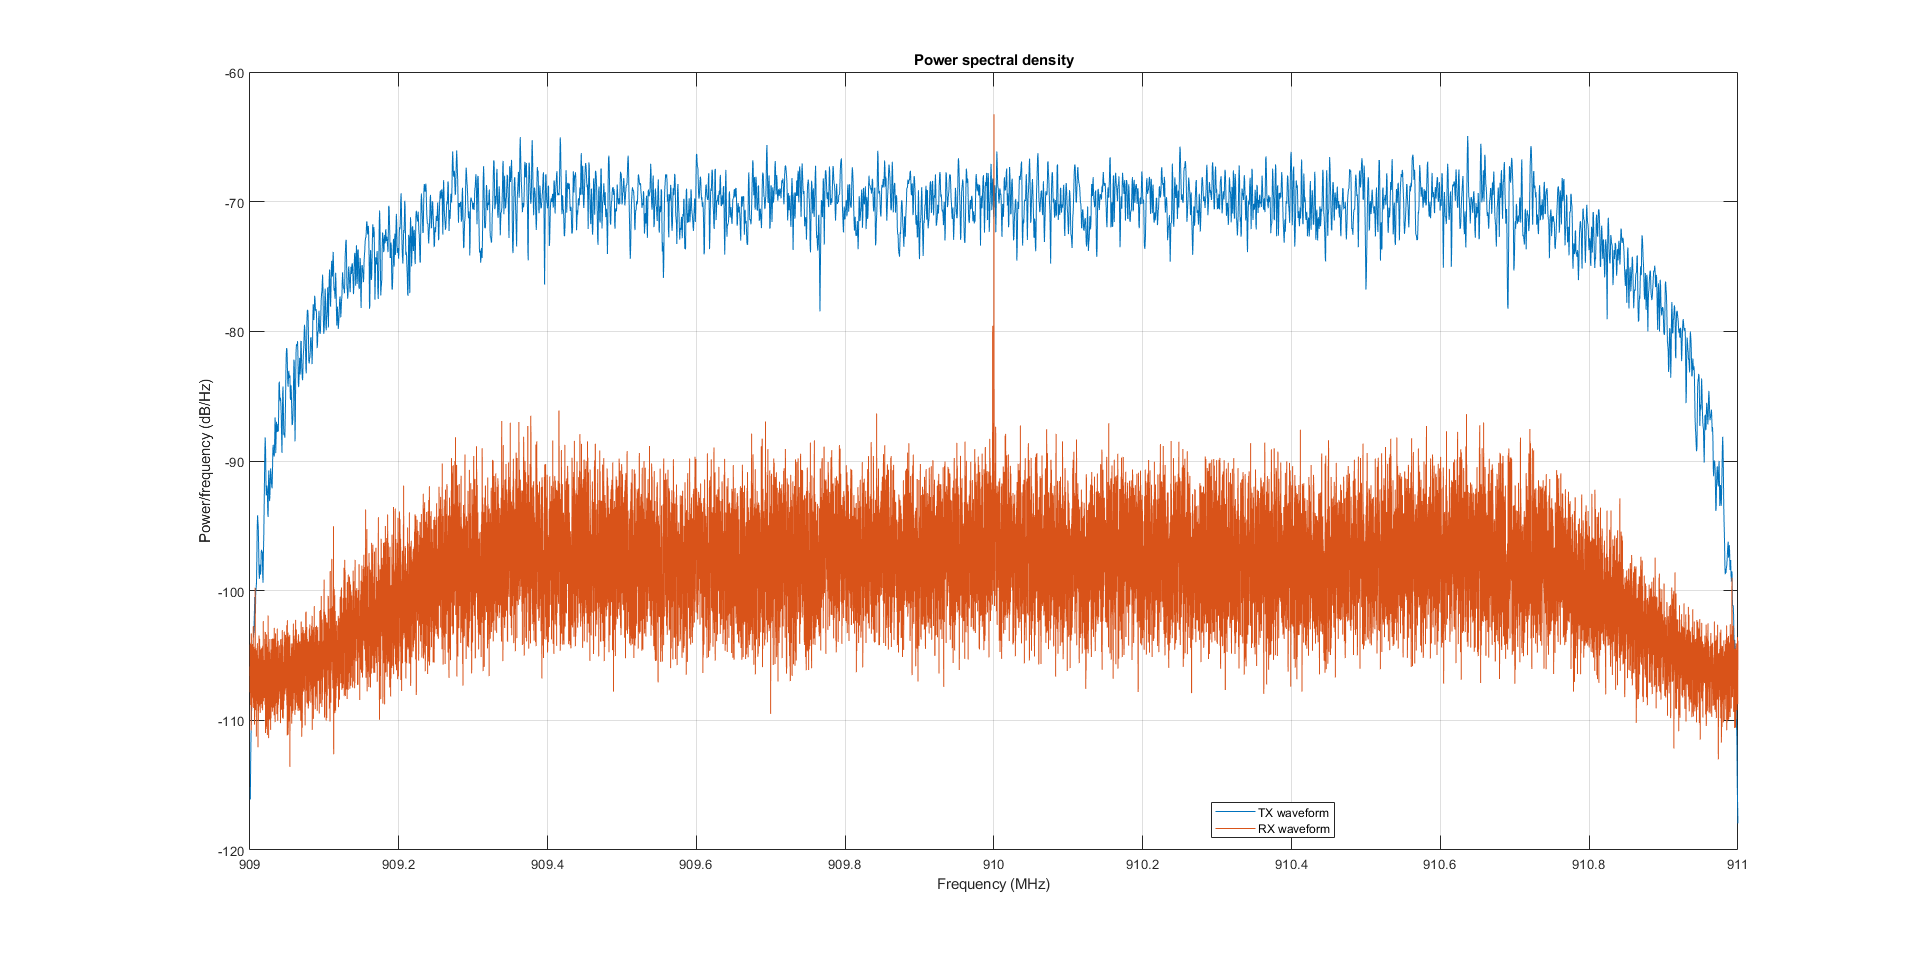
\includegraphics[width=\textwidth]{beta01_PSD.png}
    \caption{Power spectral density for $\beta = 0.1$.}
    \label{fig:beta01_PSD}
\end{figure}

\begin{figure}[h]
    \centering
    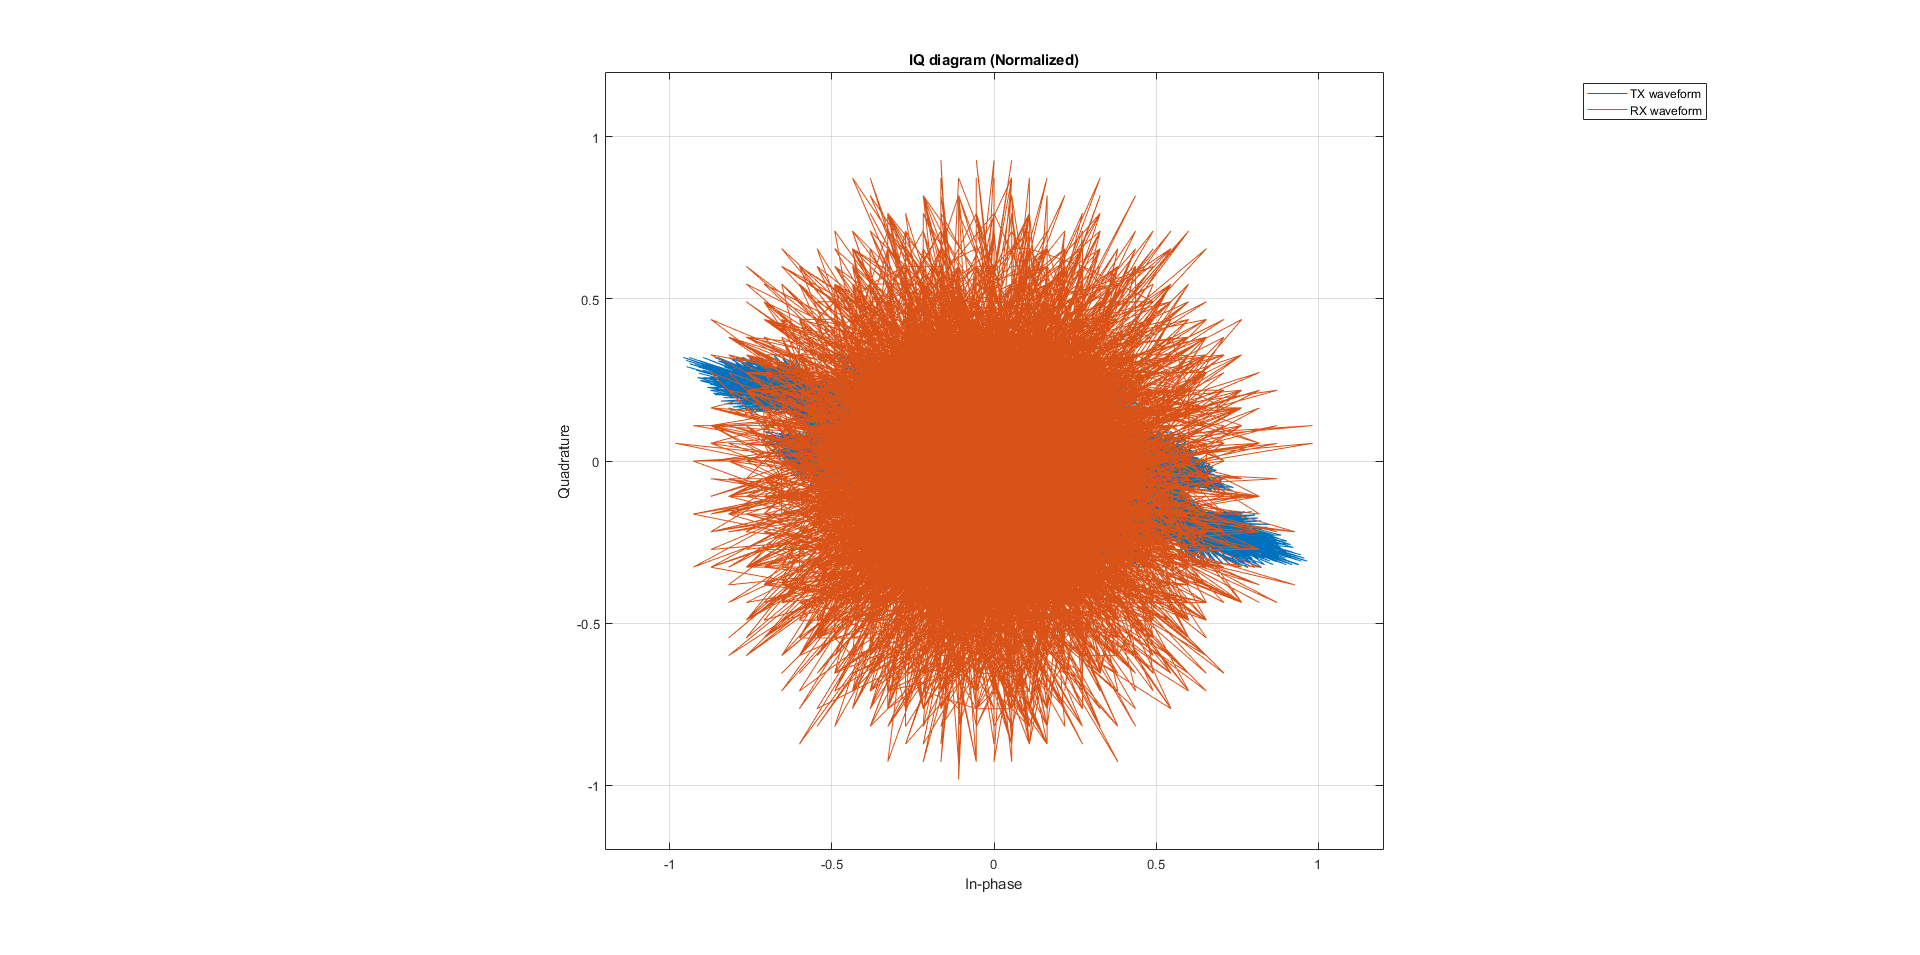
\includegraphics[width=\textwidth]{beta01_IvsQ.png}
    \caption{IQ diagram (normalized) for $\beta = 0.1$.}
    \label{fig:beta01_IvsQ}
\end{figure}

\begin{figure}[h]
    \centering
    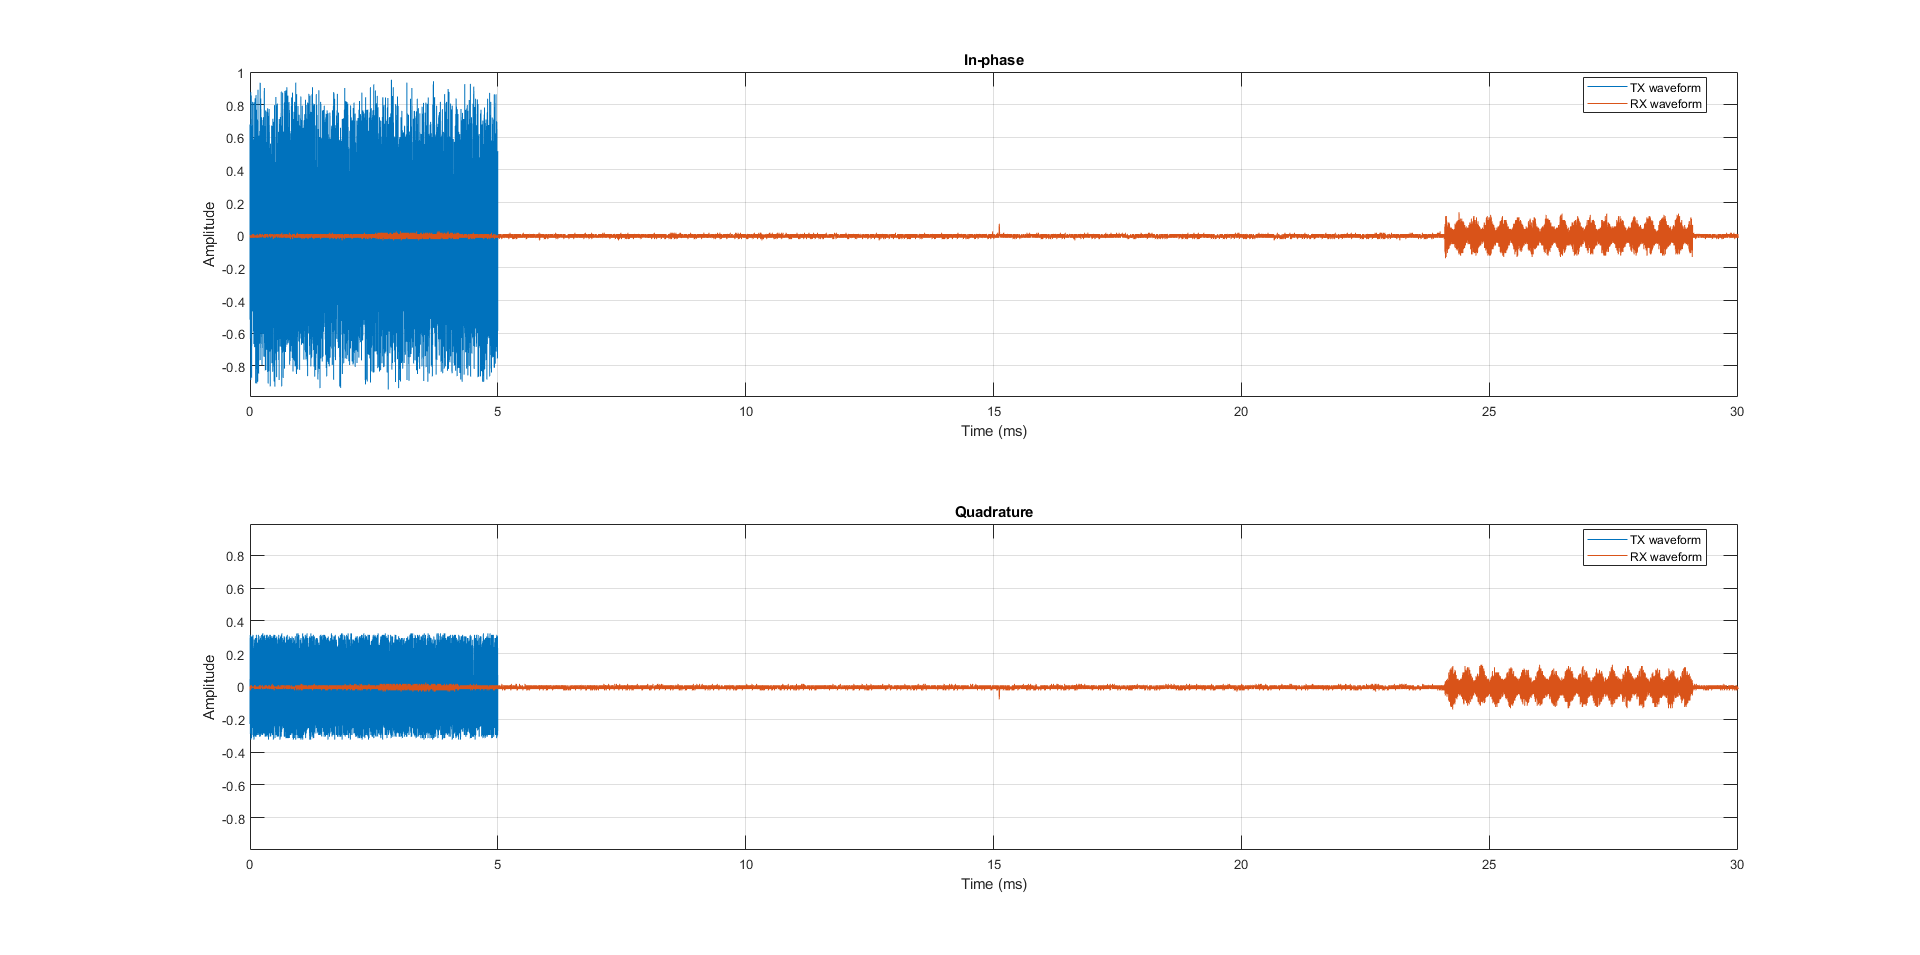
\includegraphics[width=\textwidth]{beta01_IQ_time.png}
    \caption{Time vs. IQ data for $\beta = 0.1$.}
    \label{fig:beta01_IQ_time}
\end{figure}

\begin{figure}[h]
    \centering
    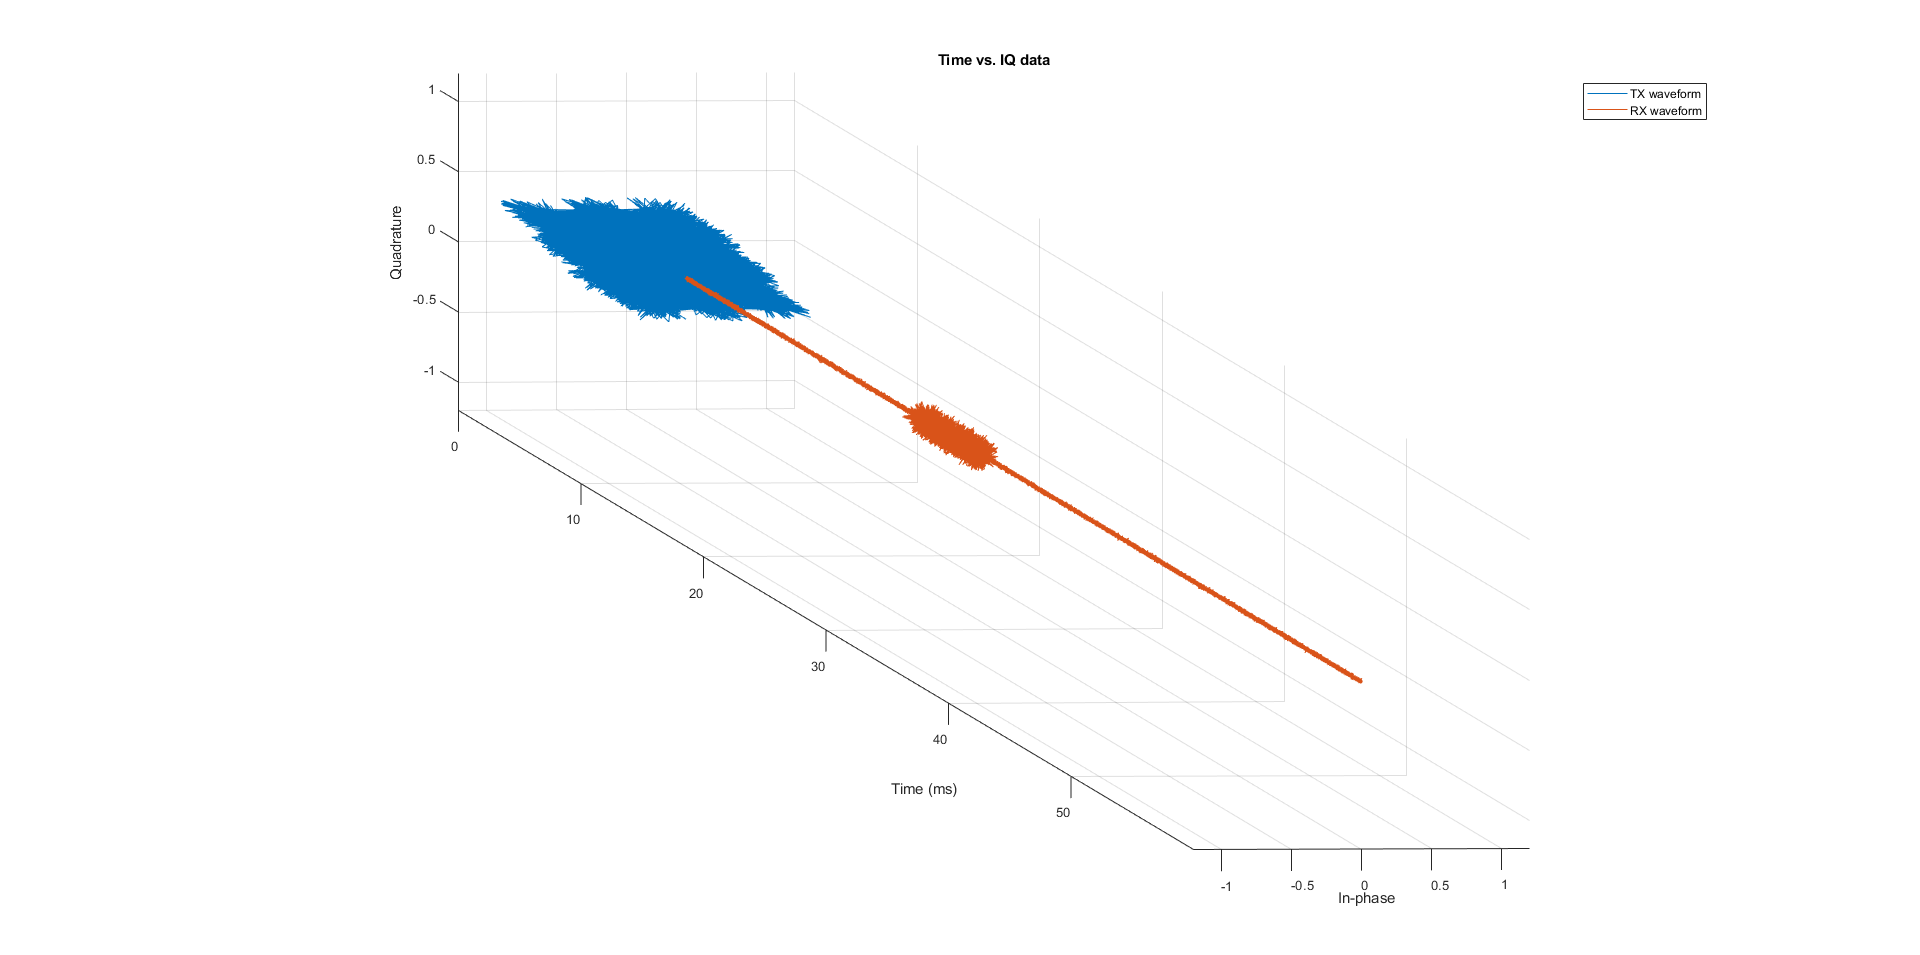
\includegraphics[width=\textwidth]{beta01_IQ_time_3d.png}
    \caption{3D Time vs. IQ data for $\beta = 0.1$.}
    \label{fig:beta01_IQ_time_3d}
\end{figure}
% Repeat for beta01_PSD.png, beta01_IQ_time_3d.png, beta01_IQ_time.png

\begin{figure}[h]
    \centering
    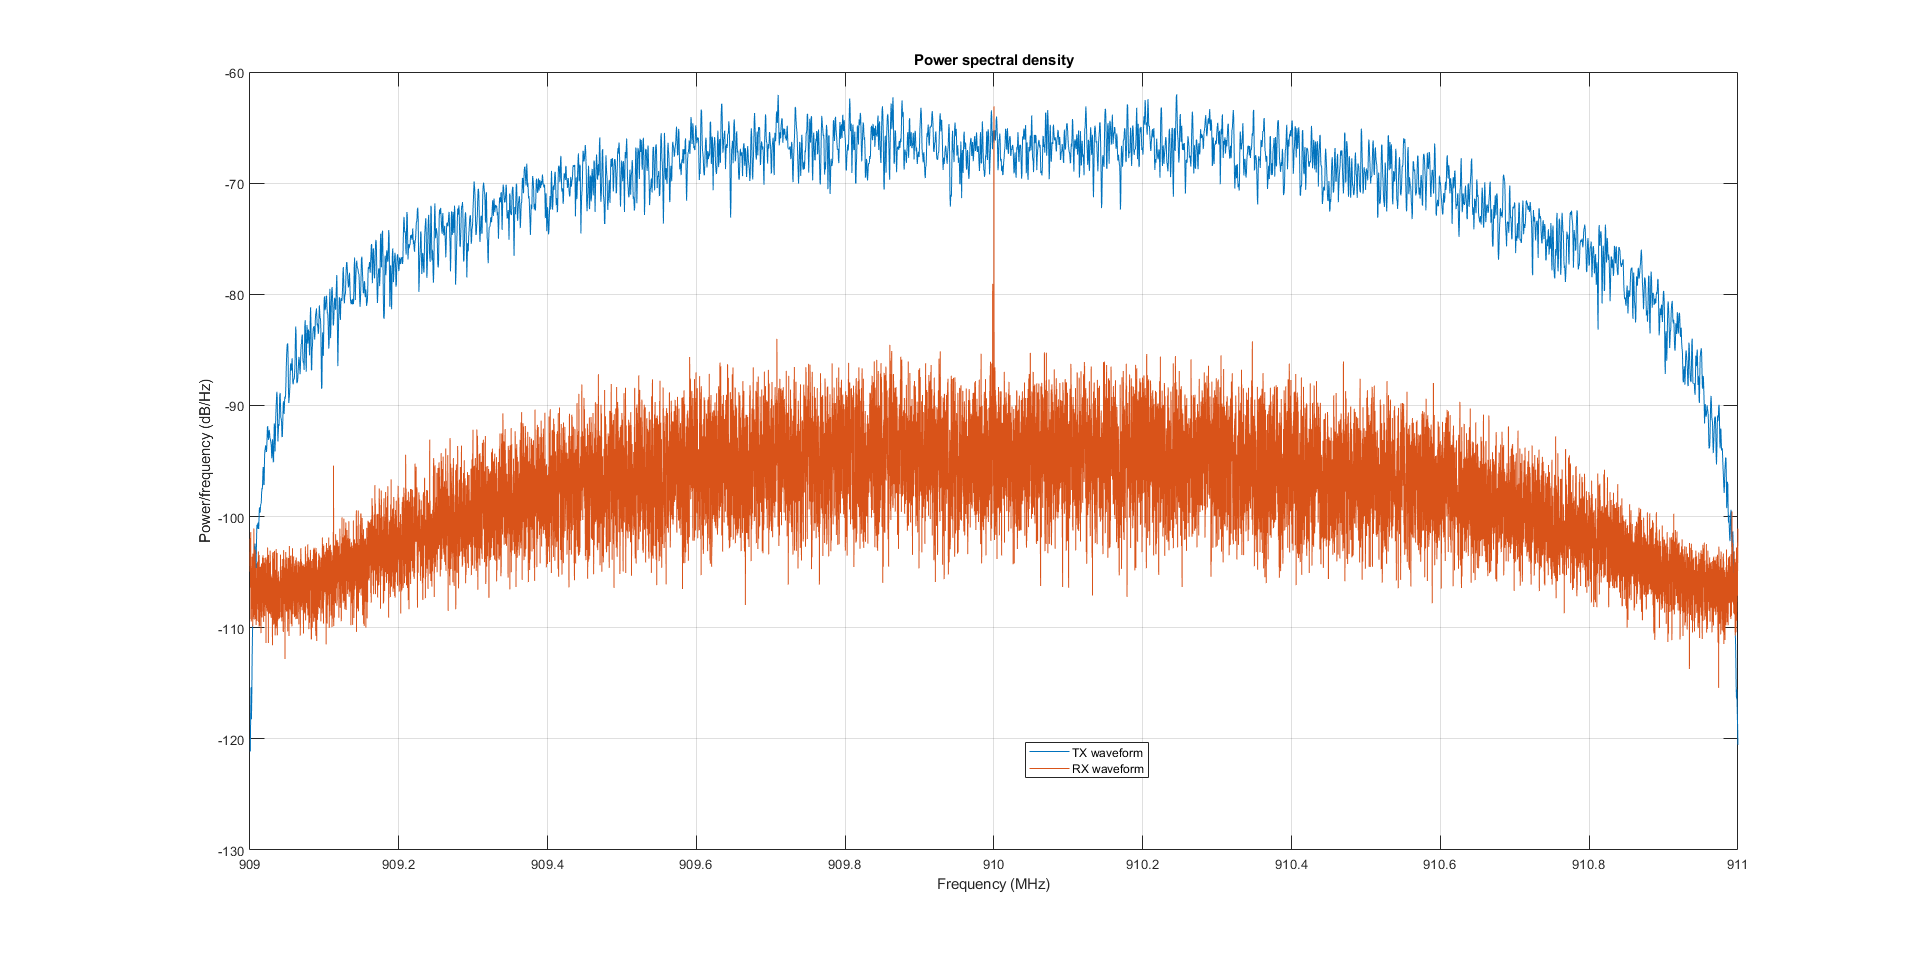
\includegraphics[width=\textwidth]{beta05_PSD.png}
    \caption{Power spectral density for $\beta = 0.5$.}
    \label{fig:beta05_PSD}
\end{figure}

\begin{figure}[h]
    \centering
    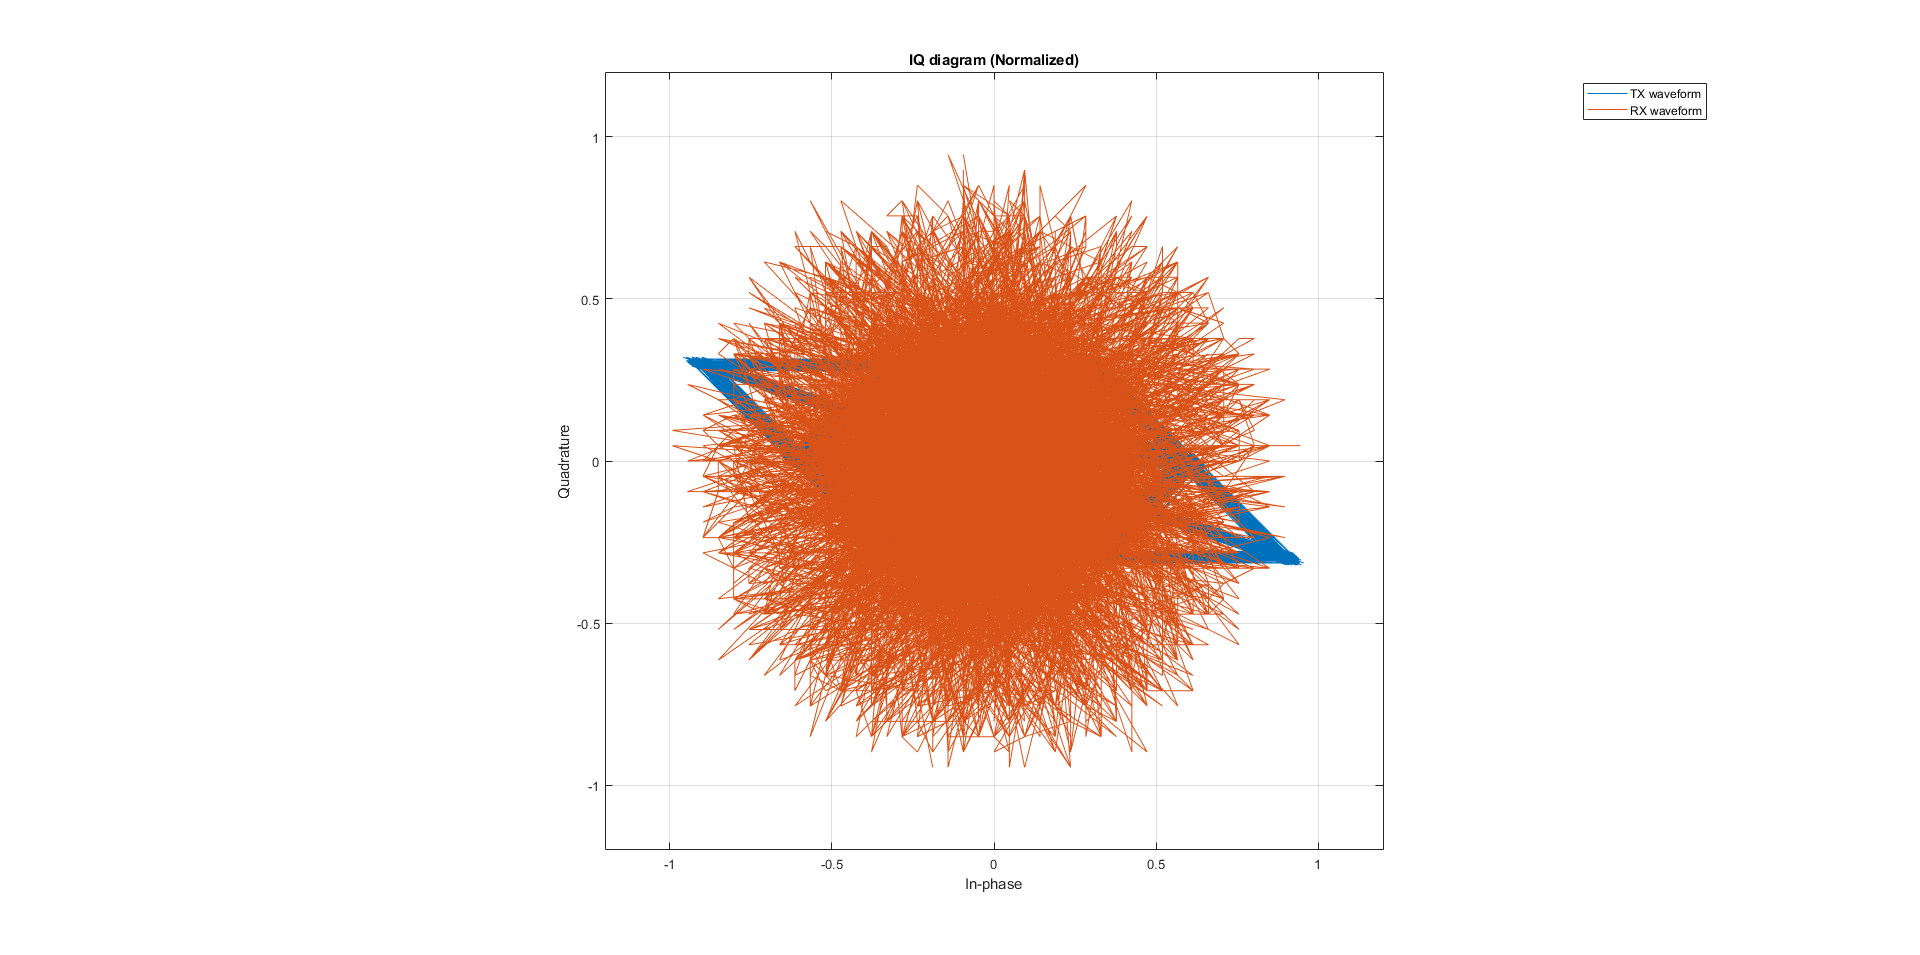
\includegraphics[width=\textwidth]{beta05_IvsQ.png}
    \caption{IQ diagram (normalized) for $\beta = 0.5$.}
    \label{fig:beta05_IvsQ}
\end{figure}

\begin{figure}[h]
    \centering
    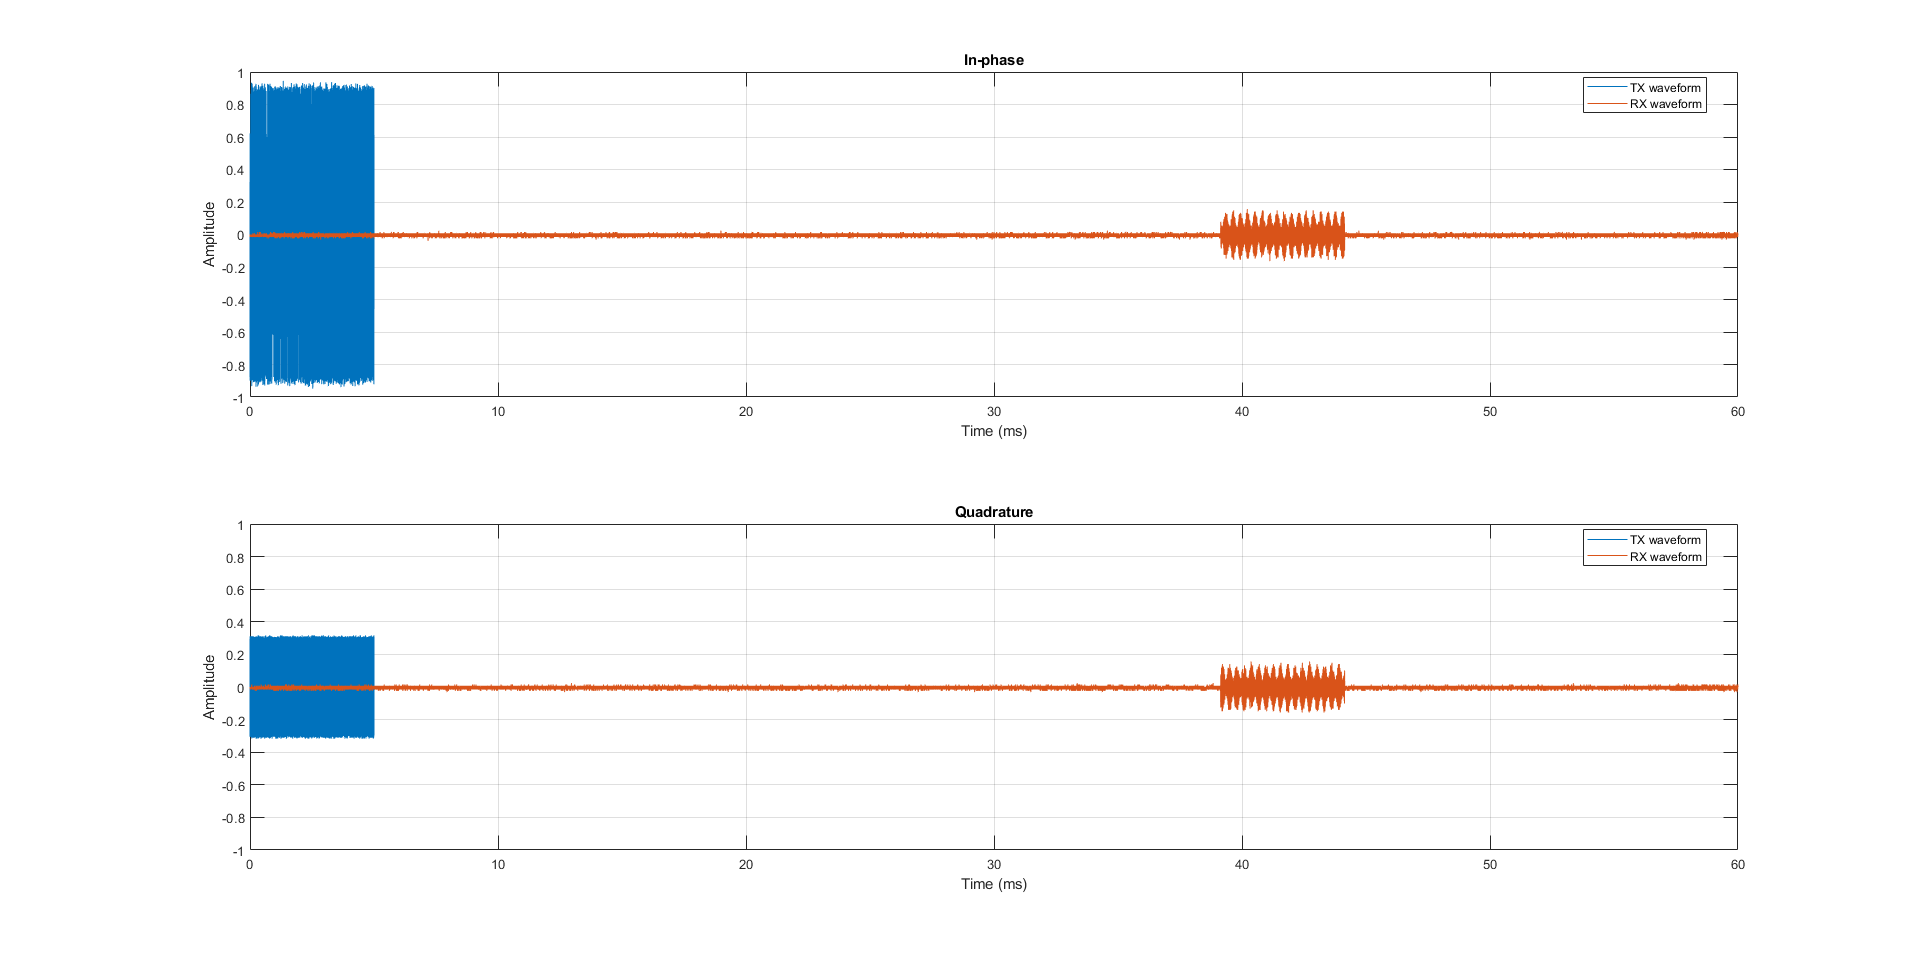
\includegraphics[width=\textwidth]{beta05_IQ_time.png}
    \caption{Time vs. IQ data for $\beta = 0.5$.}
    \label{fig:beta05_IQ_time}
\end{figure}

\begin{figure}[h]
    \centering
    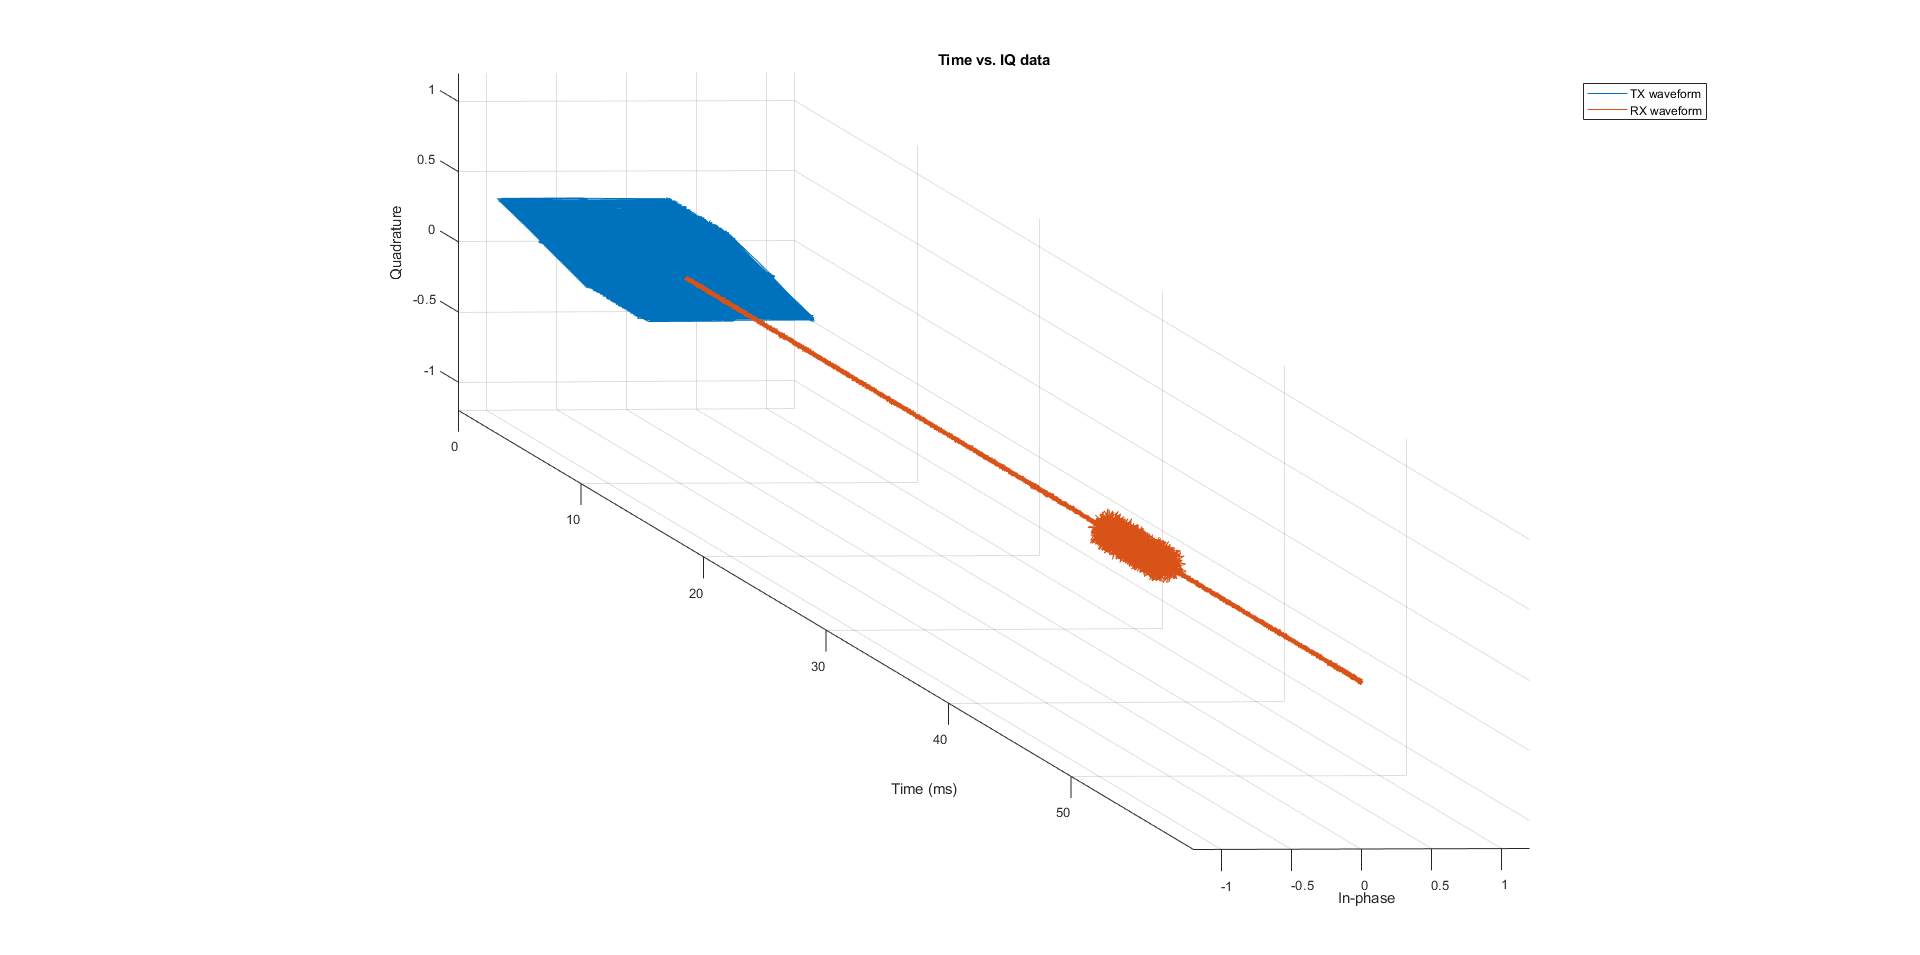
\includegraphics[width=\textwidth]{beta05_IQ_time_3d.png}
    \caption{3D Time vs. IQ data for $\beta = 0.5$.}
    \label{fig:beta05_IQ_time_3d}
\end{figure}

\begin{figure}[h]
    \centering
    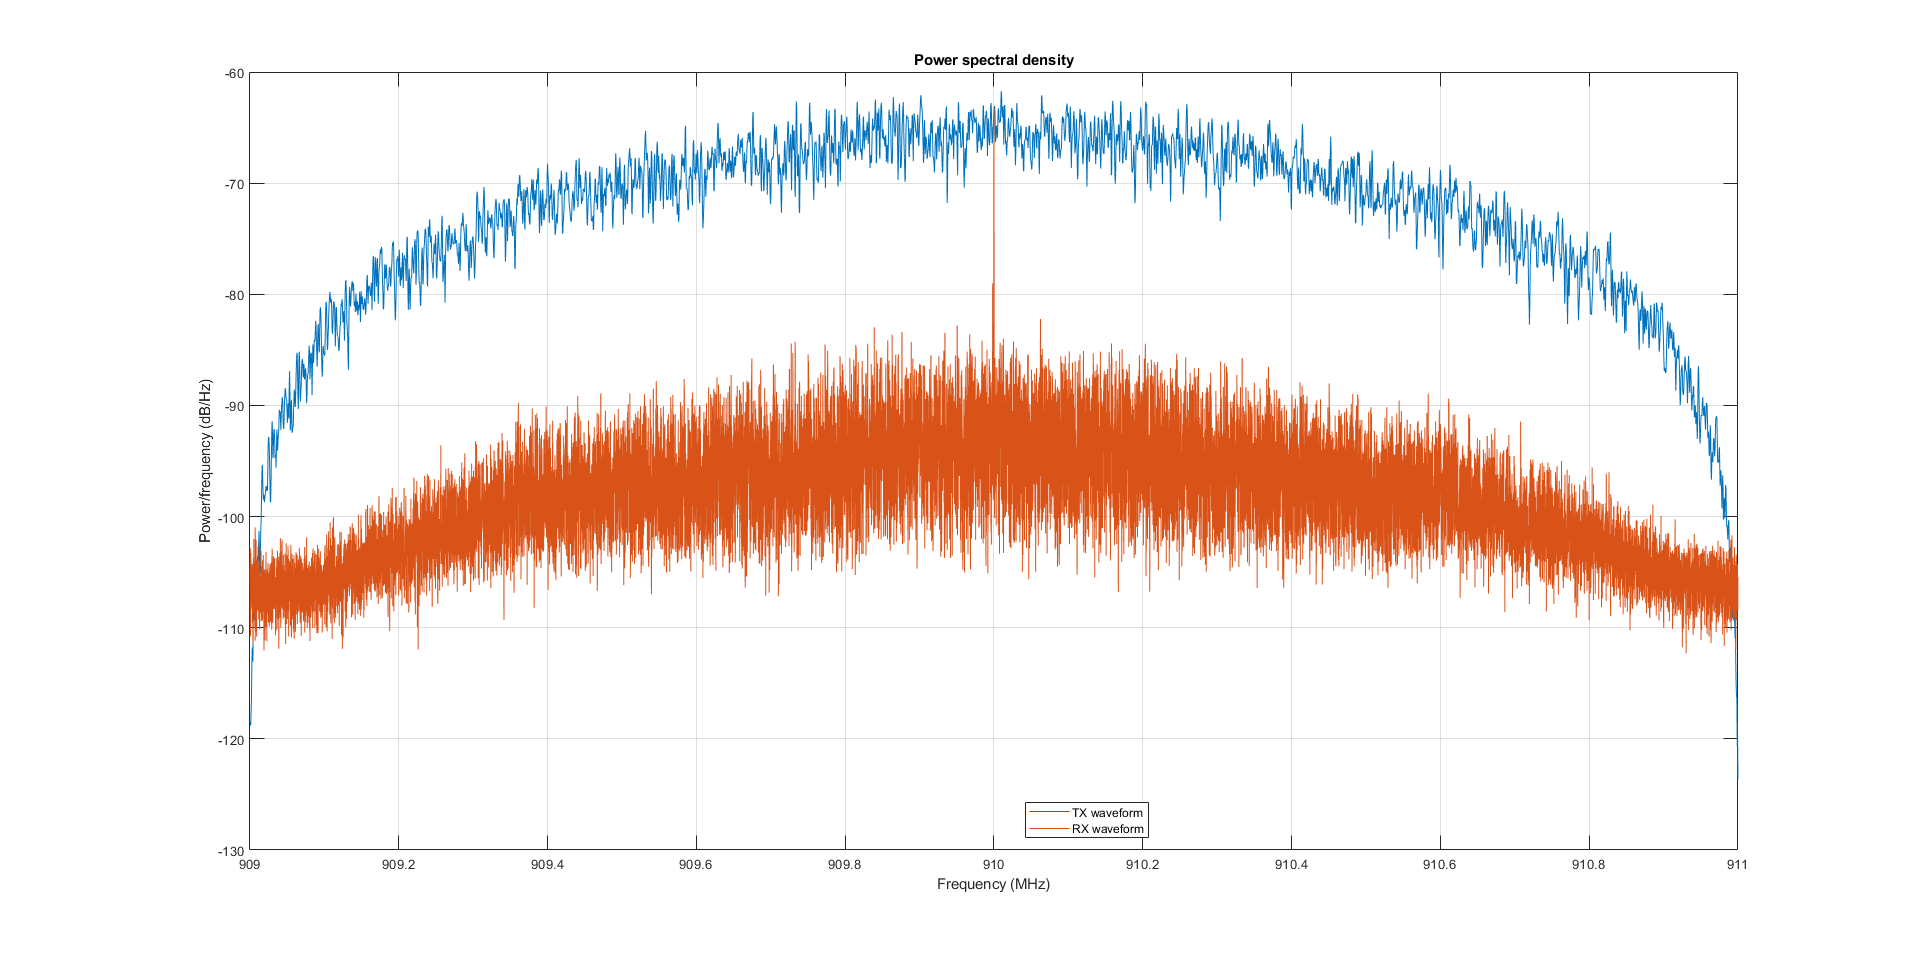
\includegraphics[width=\textwidth]{beta09_PSD.png}
    \caption{Power spectral density for $\beta = 0.9$.}
    \label{fig:beta09_PSD}
\end{figure}

\begin{figure}[h]
    \centering
    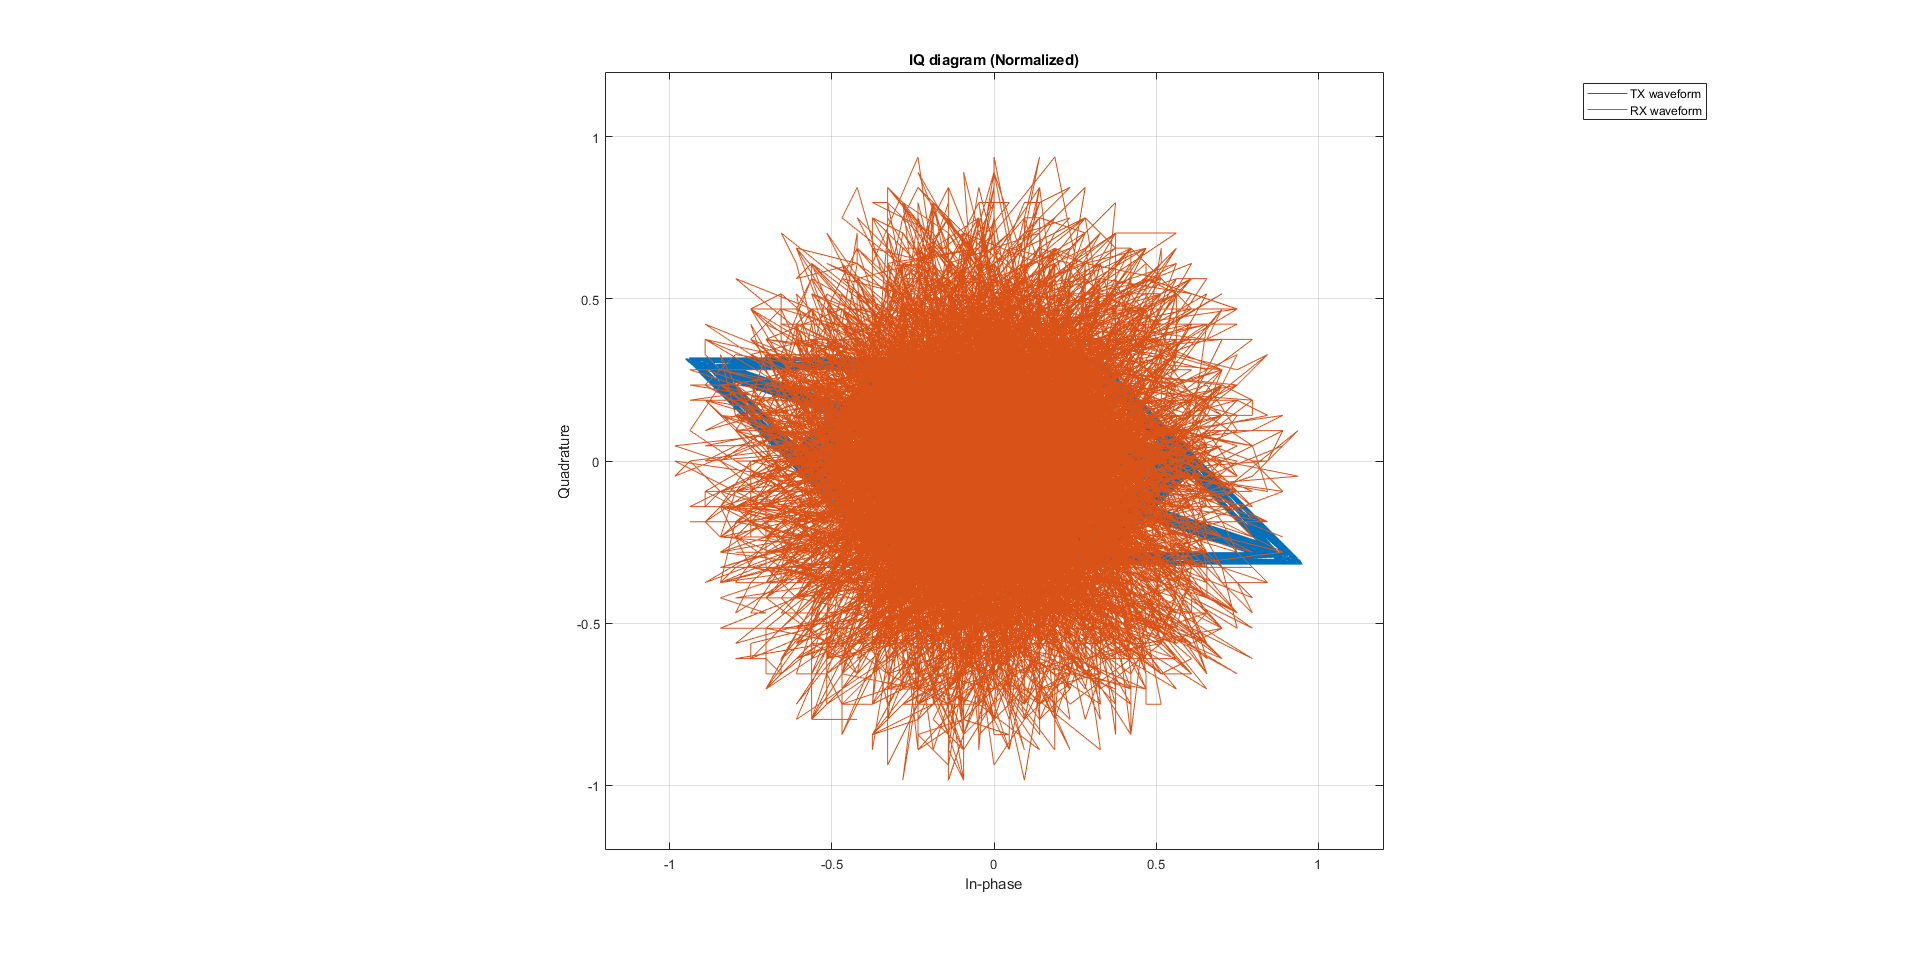
\includegraphics[width=\textwidth]{beta09_IvsQ.png}
    \caption{IQ diagram (normalized) for $\beta = 0.9$.}
    \label{fig:beta09_IvsQ}
\end{figure}

\begin{figure}[h]
    \centering
    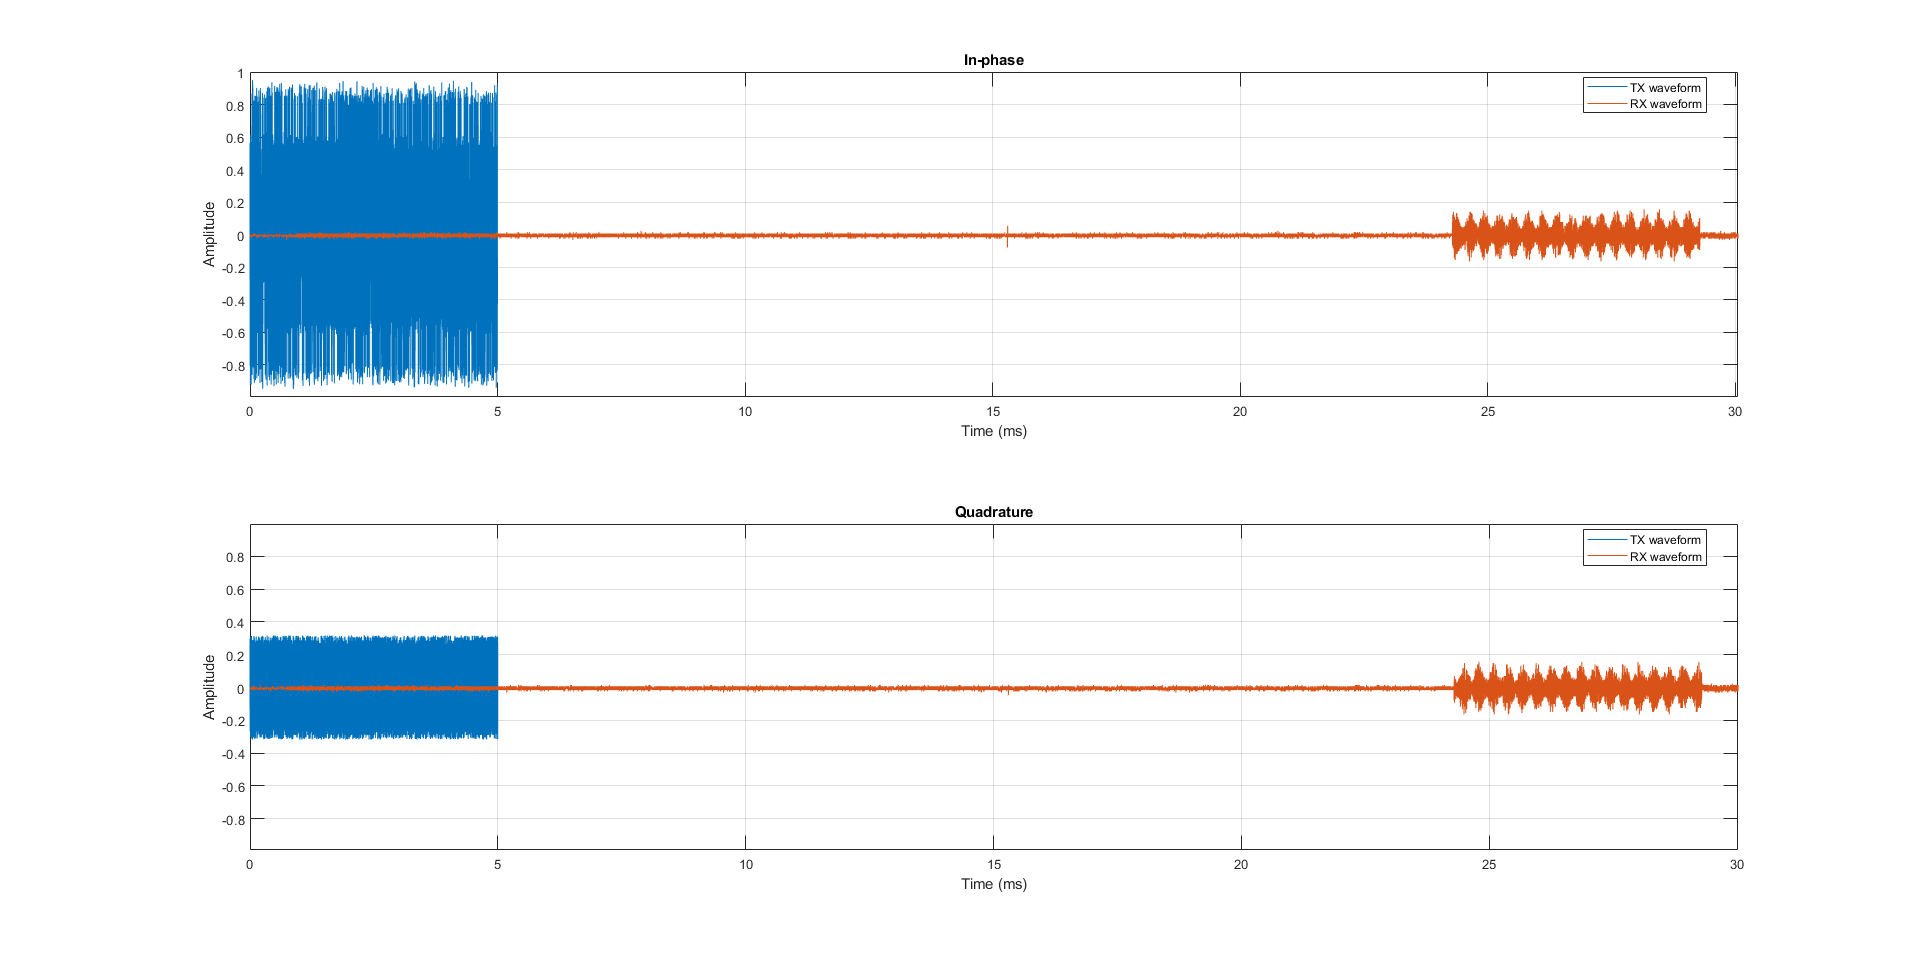
\includegraphics[width=\textwidth]{beta09_IQ_time.png}
    \caption{Time vs. IQ data for $\beta = 0.9$.}
    \label{fig:beta09_IQ_time}
\end{figure}

\begin{figure}[h]
    \centering
    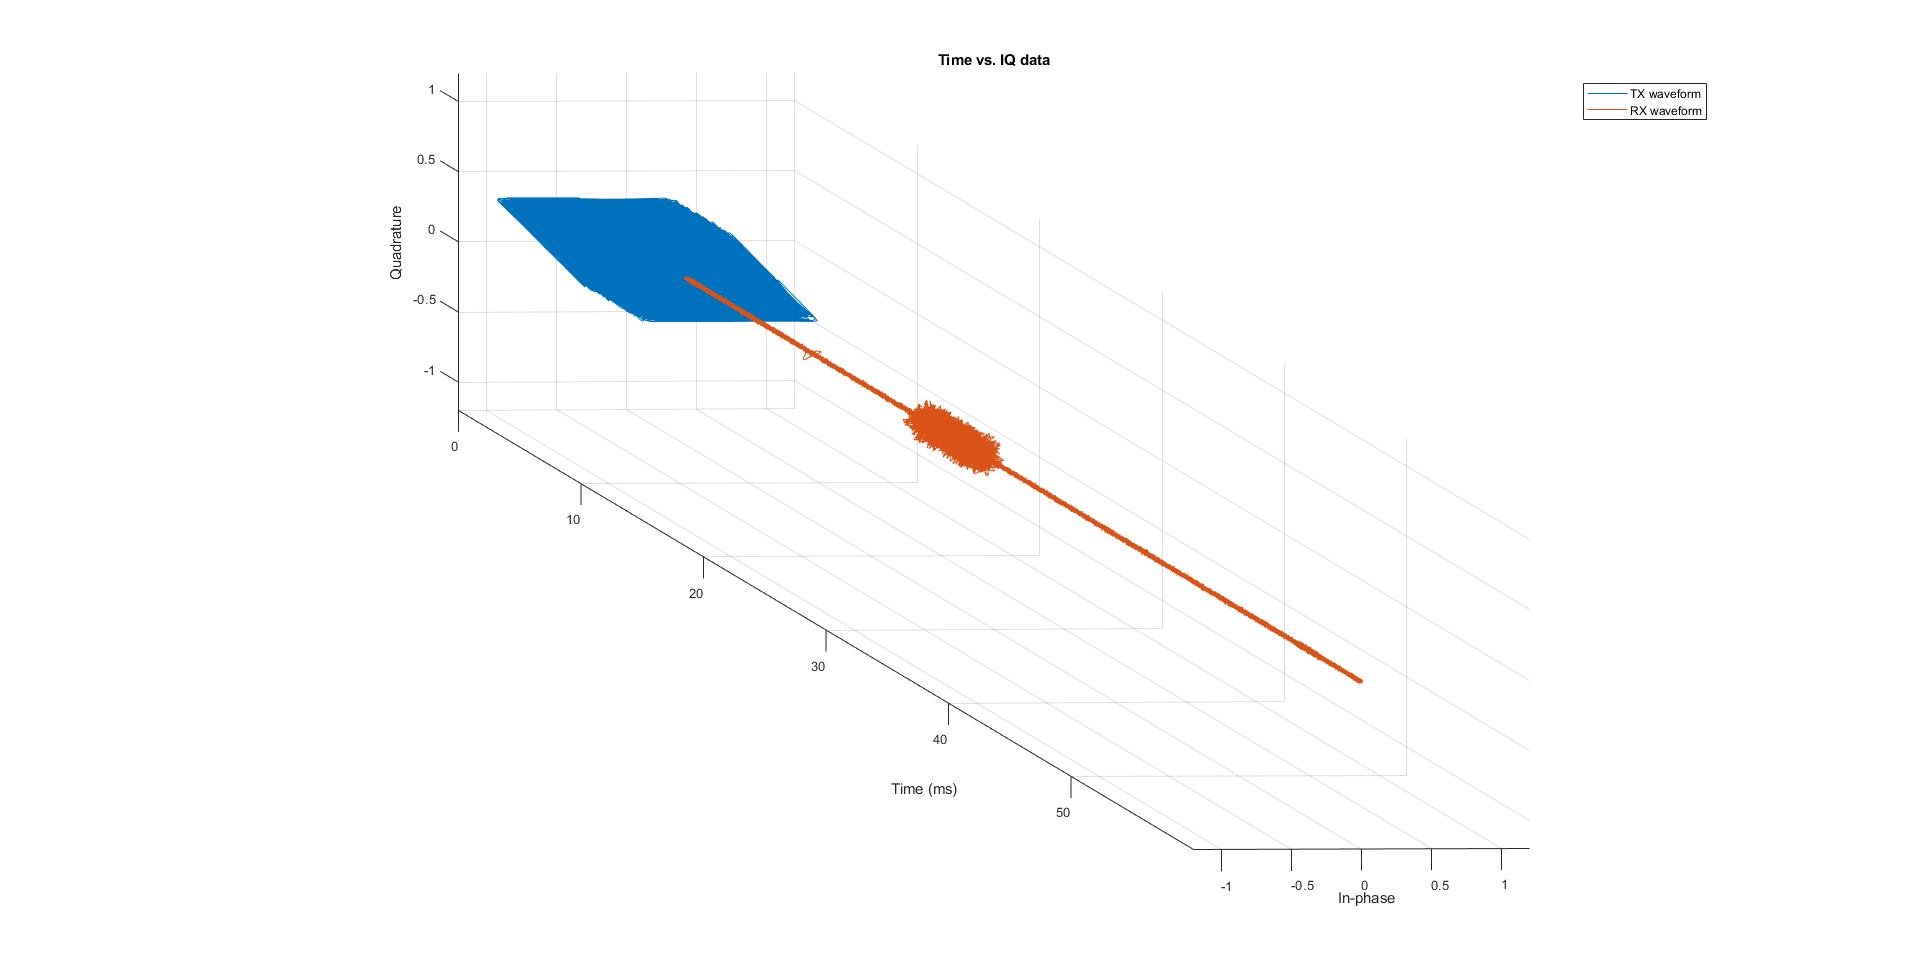
\includegraphics[width=\textwidth]{beta09_IQ_time_3d.png}
    \caption{3D Time vs. IQ data for $\beta = 0.9$.}
    \label{fig:beta09_IQ_time_3d}
\end{figure}


\end{document}
